\chapter{Elkészült funkciók tesztelése}

\section{Live streaming tesztelése}

A weboldalamon a \verb|/live| útvonalon megtekintettem az előzőleg (\ref{sec:mediaLive}. alfejezet) beindított streamet (\refstruc{fig:waterfall1}). Egy próbálkozást mutat be \az+\refstruc{fig:waterfall2} képernyőkép, amely a~böngészőben a HTTP-kérések vízesését\cite{waterfall} mutatja be.

\begin{figure}[h]
  \centering
  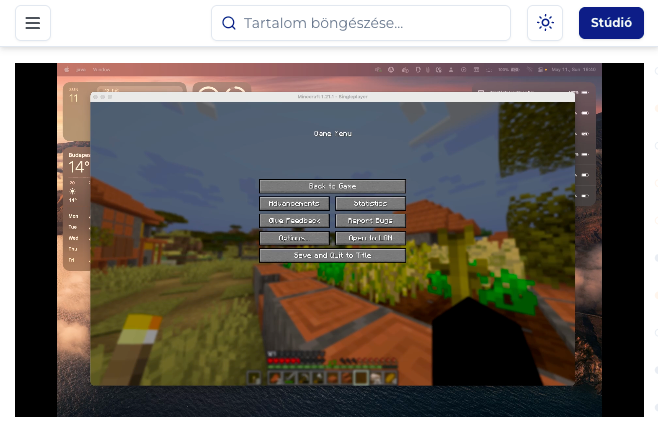
\includegraphics[width=100mm, keepaspectratio]{figures/waterfall1.png}
  \caption{A /live útvonalon látható aloldal.}
  \label{fig:waterfall1}
\end{figure}

\begin{figure}[h]
  \centering
  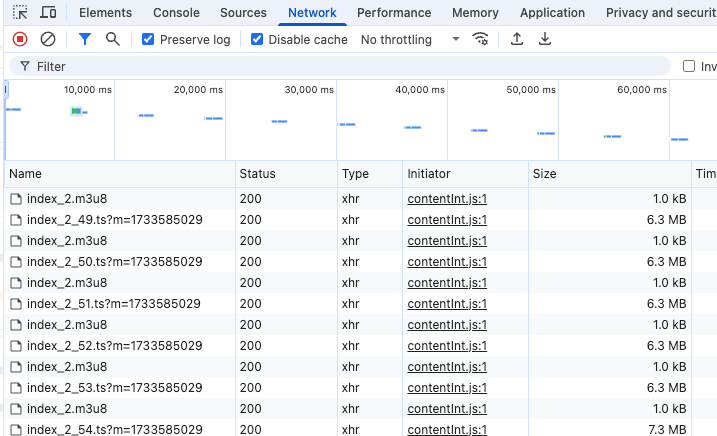
\includegraphics[width=100mm, keepaspectratio]{figures/waterfall2.png}
  \caption{HTTP-kérések vízesése a /live oldalon.}
  \label{fig:waterfall2}
\end{figure}

Az SPA-alkalmazás a környezeti változóból beállított HLS-végponton kéri le először a~\verb|.m3u8| playlistet, amelyből megtudja, mi lesz a következő szegmens, amelyet le kell töltse. Az ábrából látszik, hogy az alapértelmezett 6 másodperces részekre vannak felbontva a~szegmensek. Nagyjából 6--7 MB-os szegmensek érkeznek a böngészőbe (már tömörítve a~CDN-en keresztül).

A MediaPackage v2-es verziója támogatja a Low Latency HLS (LL-HLS) alapú streamelést is, azonban én még a v1-es verziót használtam és a kliensoldali implementációs is meghagytam a hagyományos HLS-en. A fent ismertetett élő stream MediaLive és MediaPackage közti integrációjának manuális tesztelése folyamán körülbelül 10 másodperces késleltetést érzékeltem.

Teljesítmény szempontjából a fenti streamelés késleltetését két dolog befolyásolja jelentősen: a kódolási beállítások (mekkora szegmensekre bontsa, hányféle kimenet legyen, milyen hibaaránnyal érkezik a forrásvideó) és a lejátszó bufferelési logikája. Előbbi befolyásoló tényezőnek a mögöttes forrása a MediaLive maga, ami a kódolást intézi. Mind a~MediaLive és a MediaPackage menedzselt szolgáltatások, magunk nem tudunk hatással lenni az azalatti erőforrások eloszlására, annak növelésére, ugyanis automatikusan skálázódnak, ahogy arra a szolgáltatás elköteleződik is.

A késleltetés mérésére a nézők számának növelésével nem tudnánk hasznos teljesítményteszteket készíteni, a live betöltődik a MediaLive-ba, utána a kész szegmensek kiszórása az, ami kihívás a rendszer számára, viszont ezt ahogy fentebb kifejtettem, a~MediaPackage automatikusan skálázódással oldja meg bizonyos kvótákig -- például egy HLS-végponton másodpercenként 300 kérést tud befogadni\cite{empQuotas} --, de még ennek a terhelését is hívatott megvédeni megfelelő gyorsítótárazással egy CDN. Csupán abban az esetben érheti teljesítményromlás a rendszert, ha a MediaPackage hatáskörén kívül magára az AWS hálózatára fejtenek ki jelentős terhelést a felhasználók.\cite{latency}

\section{VOD streaming tesztelése}\label{sec:vod_test}

A VOD streameket közvetlen S3-ból szolgáljuk ki. A technológiai ismertető (\ref{sec:aws_elemental}. alfejezet) is referált már rá, korábban a videók tárolására a széleskörű kiszolgálásra korábban létezett szolgáltatás, azonban ezt kiváltotta az S3.\cite{Mediastore} Az S3 szintén fel van készítve a skálázódásra\cite{s3perf}, így nem szükséges aggódni, viszont a kiszolgálás késleltetését érdemes csökkenteni úgy, hogy az edge rétegén gyorsítótárazást valósítunk meg, ezt persze CDN-nel. A CloudFront cache beállításaival való kísérletezésre összeállítottam egy tesztkörnyezetet, amelyben a CDN cache beállításait variálva figyeltem meg a válaszidőket. A teszteléshez a \emph{Grafana k6}-ot\footnote{\url{https://k6.io/}} használtam, amelynek segítségével a válaszidőket és a válaszok méretét is tudtam mérni.\cite{loadtests}

Nyilván egy 1 éves caching policy bekapcsolásával a \verb|/media-assets| elérési útvonalra érkező kérések válaszideje csökkent, hiszen az adatok a CDN gyorsítótárából, konkrétan a~budapesti edge szerverfarmról érkeztek, nem pedig közvetlenül az S3-ból, amely a~frankfurti adatközpontban lakik. A tesztelés alatt 100 virtuális felhasználó egy megadott kétperces ablakban alatt szórt felhasználónként 20 kérést, vegyesen kérték le egy videó szegmenseit. A szkript kódját mutatja be \az+\ref{lst:k6}. kódrészlet. A tesztelés során cache nélkül a válasz megérkezésére a várakozási idő az esetek 90\%-ában 226,59 ms vagy azalatti volt, míg ugyanez a cache beállítással 177,39 ms vagy azalatti volt.

\begin{minipage}{0.92\textwidth}
  \begin{lstlisting}[
    caption=A k6 tesztelő szkript kódja.,
    label=lst:k6,
    style=tf,
    basicstyle=\fontsize{10}{12}\ttfamily,
  ]
export const options = {
  scenarios: {
    contacts: {
      executor: 'per-vu-iterations',
      vus: 100,
      iterations: 20,
      maxDuration: '2m',
    },
  },
};
const basePath = "https://stream.trisz.hu/media-assets";
const videoPath = basePath + "/cmajngfey0005hadzcbli5k2c/2025-05-11T12-48-43.mp4_1080p_";

export default function() {
  const n = Math.floor(Math.random() * 11) + 1; // 1-11
  const res = http.get(videoPath + String(n).padStart(5, '0') + '.ts');
  check(res, {
    'is status 200': (r) => r.status === 200,
    'is loaded': (r) => r.body.length > 0,
    'is cached': (r) => r.headers['X-Cache'] === 'Hit from cloudfront',
  });
}  
\end{lstlisting}
\end{minipage}
